\documentclass[../../main.tex]{subfiles}

 \lhead{Implementation: Real RIR Measurements}
 
\begin{document}

\subsection{Real RIR Recordings}
\label{realRIRs}
	
%-------------RIR Setup-------------%
	\subsubsection{RIR Measurement Setup}

		For the \ac{VSS} it is desirable to obtain \ac{RIR}'s that can be used to represent the topology of a singer, i.e mouth (sound source) bellow the ears (receiver). To achieve this, a Genelec 8040B \cite{genelec} loudspeaker was used as a directional sound source and a Soundfield St450 MKII microphone \cite{st450} was used as the receiver to record the three dimensional sound field in Ambisonic B-format. 

		Figure~\ref{realRIRTop} shows an image of the human head topology sound source and receiver set up. The Genelec is placed 1m above the ground (from the bas of the speaker to the floor) and the Soundfield microphone places 0.6m above the sound source. Ideally the receiver would be placed closer to the sound source to more accurately represent the distance between the ears and the mouth, however due to the physical dimensions of the equipment being used this was not possible. The sound source was placed 1m off the ground simply due to the limitations set by the maximum height of the microphone stand.

		Figure~\ref{realRIRSetup} shows the overall set up used for recording the \ac{RIR}'s as follows: \textbf{(1)} the Genelec and Soundfield microphone in the above mentioned source and receiver set up with a special soundfield cable running into \textbf{(2)}, the soundfield unit used to output a 4 channel B-format signal through 4 XLR to jack cables to \textbf{(3)} a Fireface UXC audio interface plugged into \textbf{(4)} a Mac running the digital audio workstation Reaper. Reaper was used to record directly to 4 channel tracks where channels 1 - 4 recorded the W, X, Y, Z channels respectively and to simultaneously output a 15 second long sinusoidal sweep to the Genelec. This method avoided synchronisation issues often faced when using separate devices to output a signal and to record a signal.

		%-------------Topology Image-------------%
		\begin{figure}[H]
			\begin{center}
				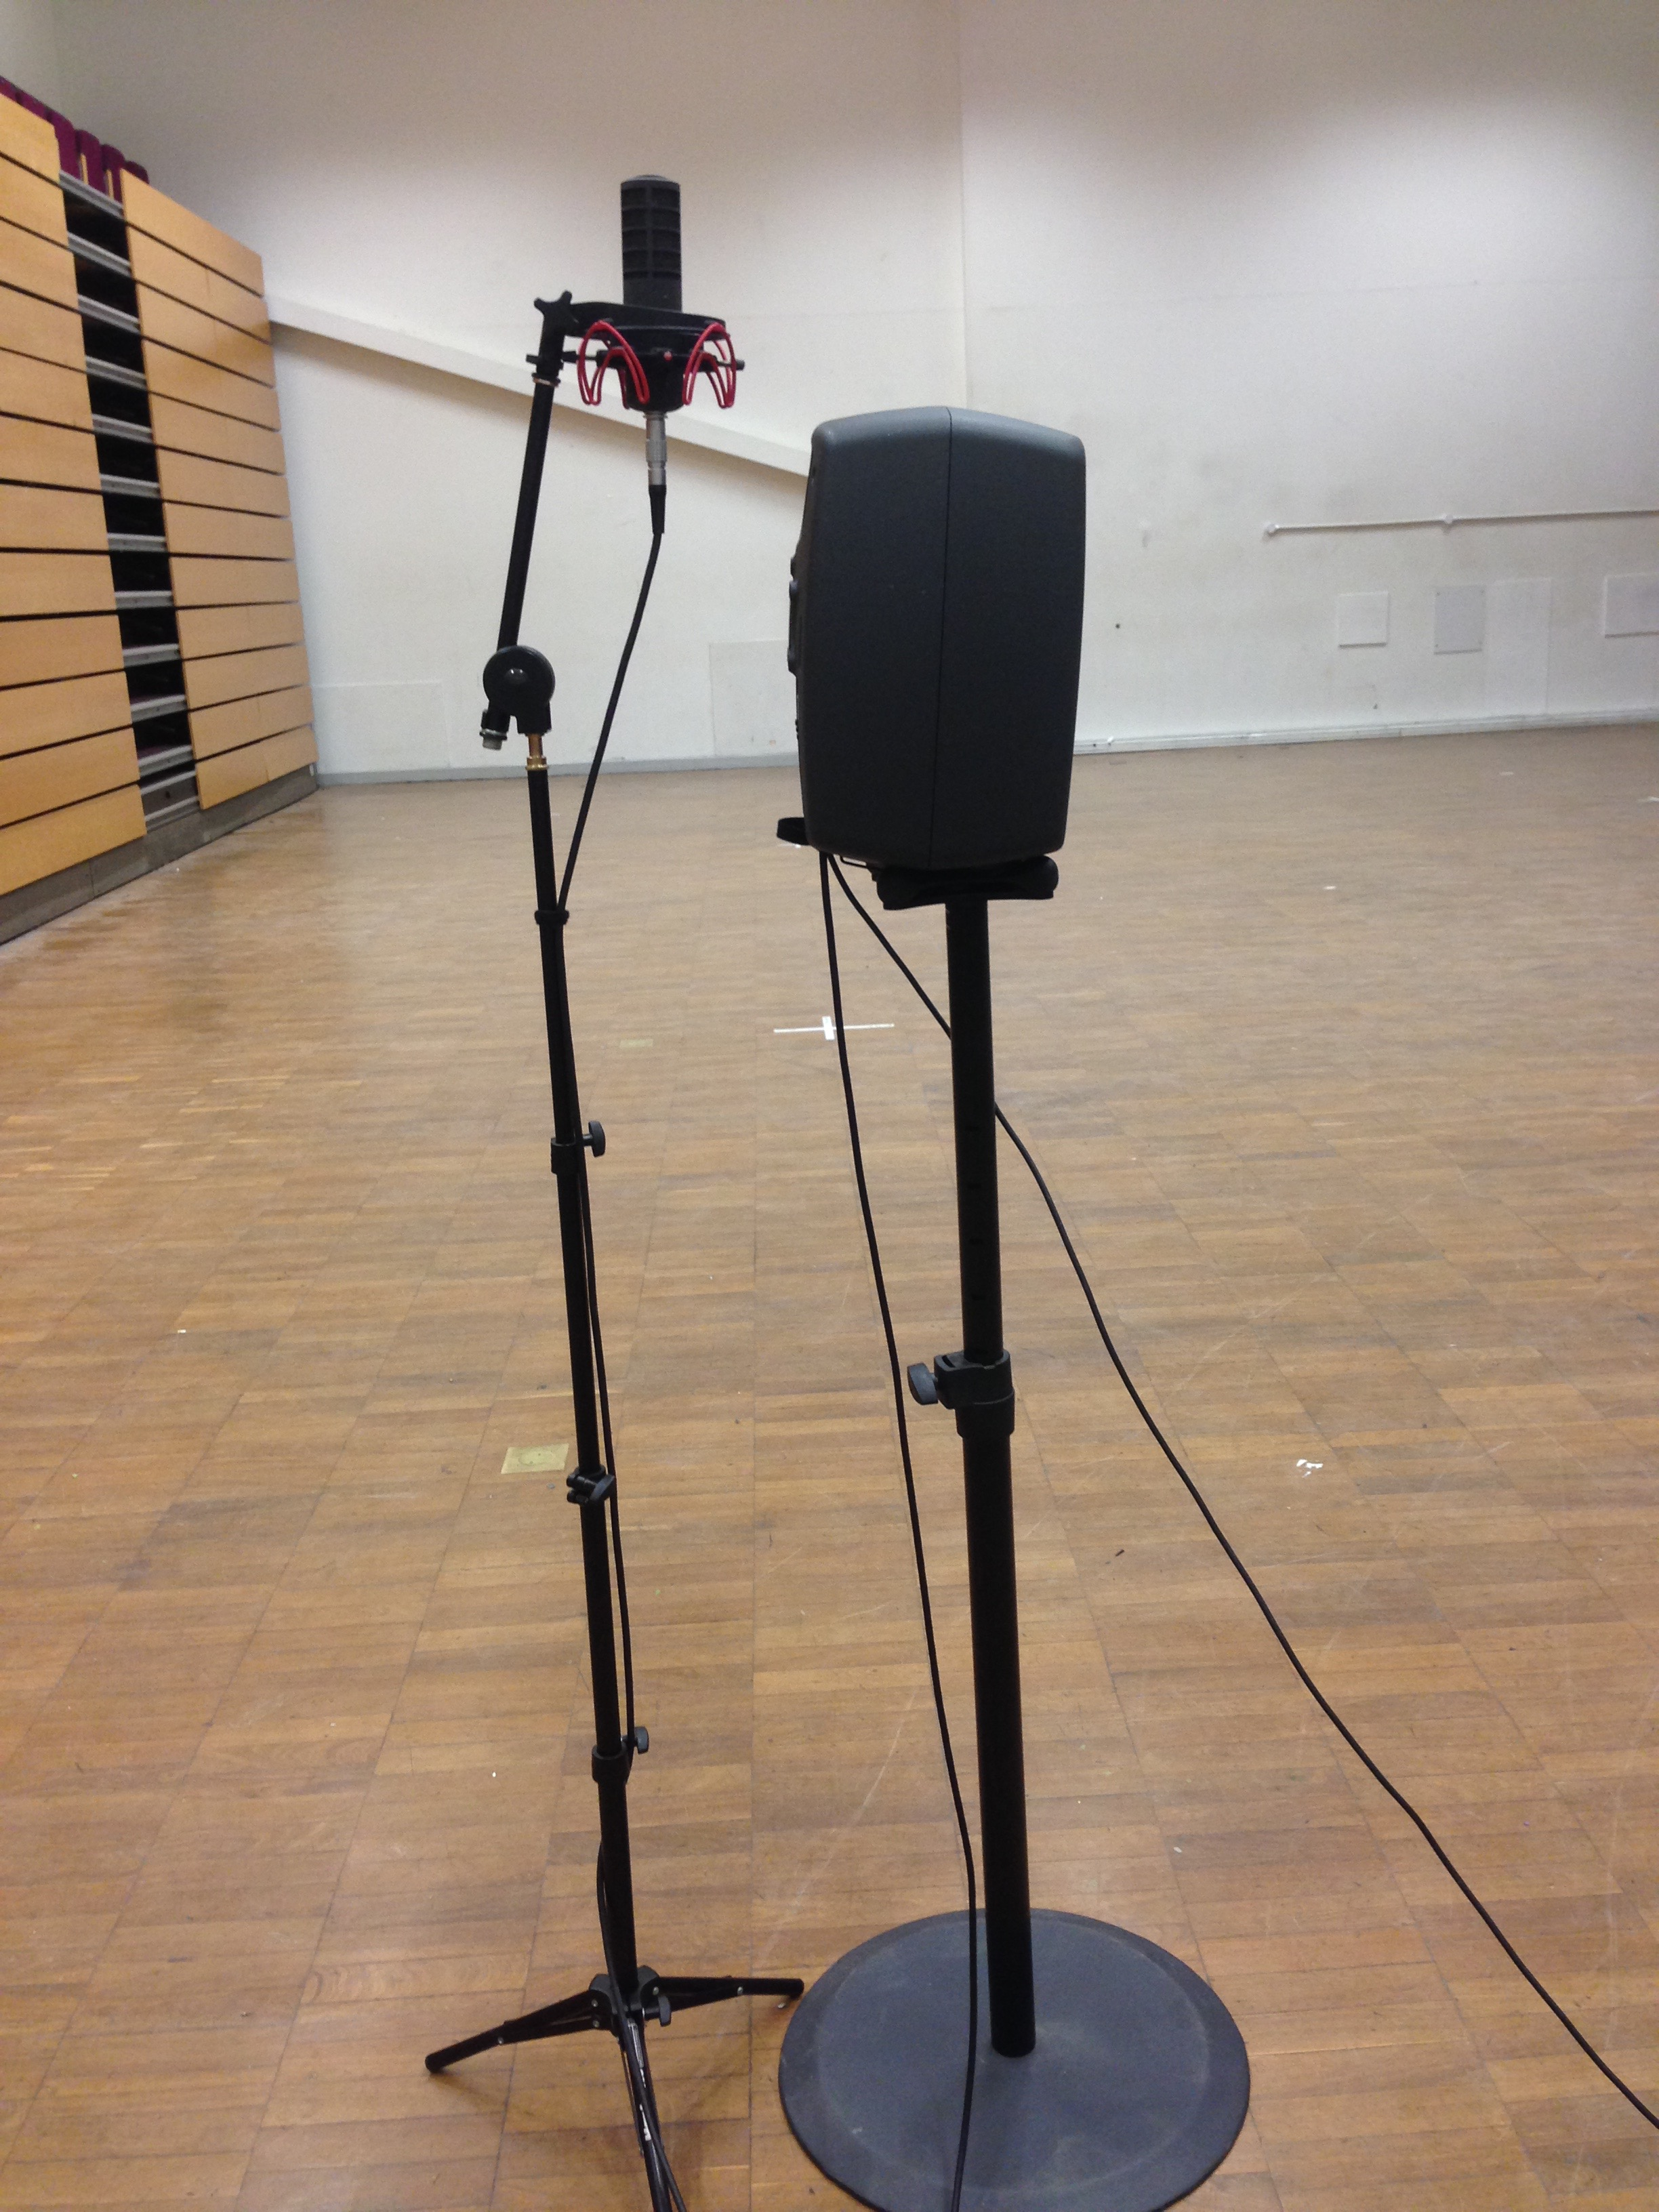
\includegraphics[scale = 0.06]{Sections/Implementation/RealRIRs/images/realRIRTopology1.jpg} 
				\caption{Human head topology \ac{RIR} measurement set up with a Genelec 8040B sound source placed 1m off the floor 0.6m below a Soundfield microphone used as a receiver}
				\label{realRIRTop}
			\end{center}
		\end{figure}

		%-------------Setup-------------%
		\begin{figure}[H]
			\begin{center}
				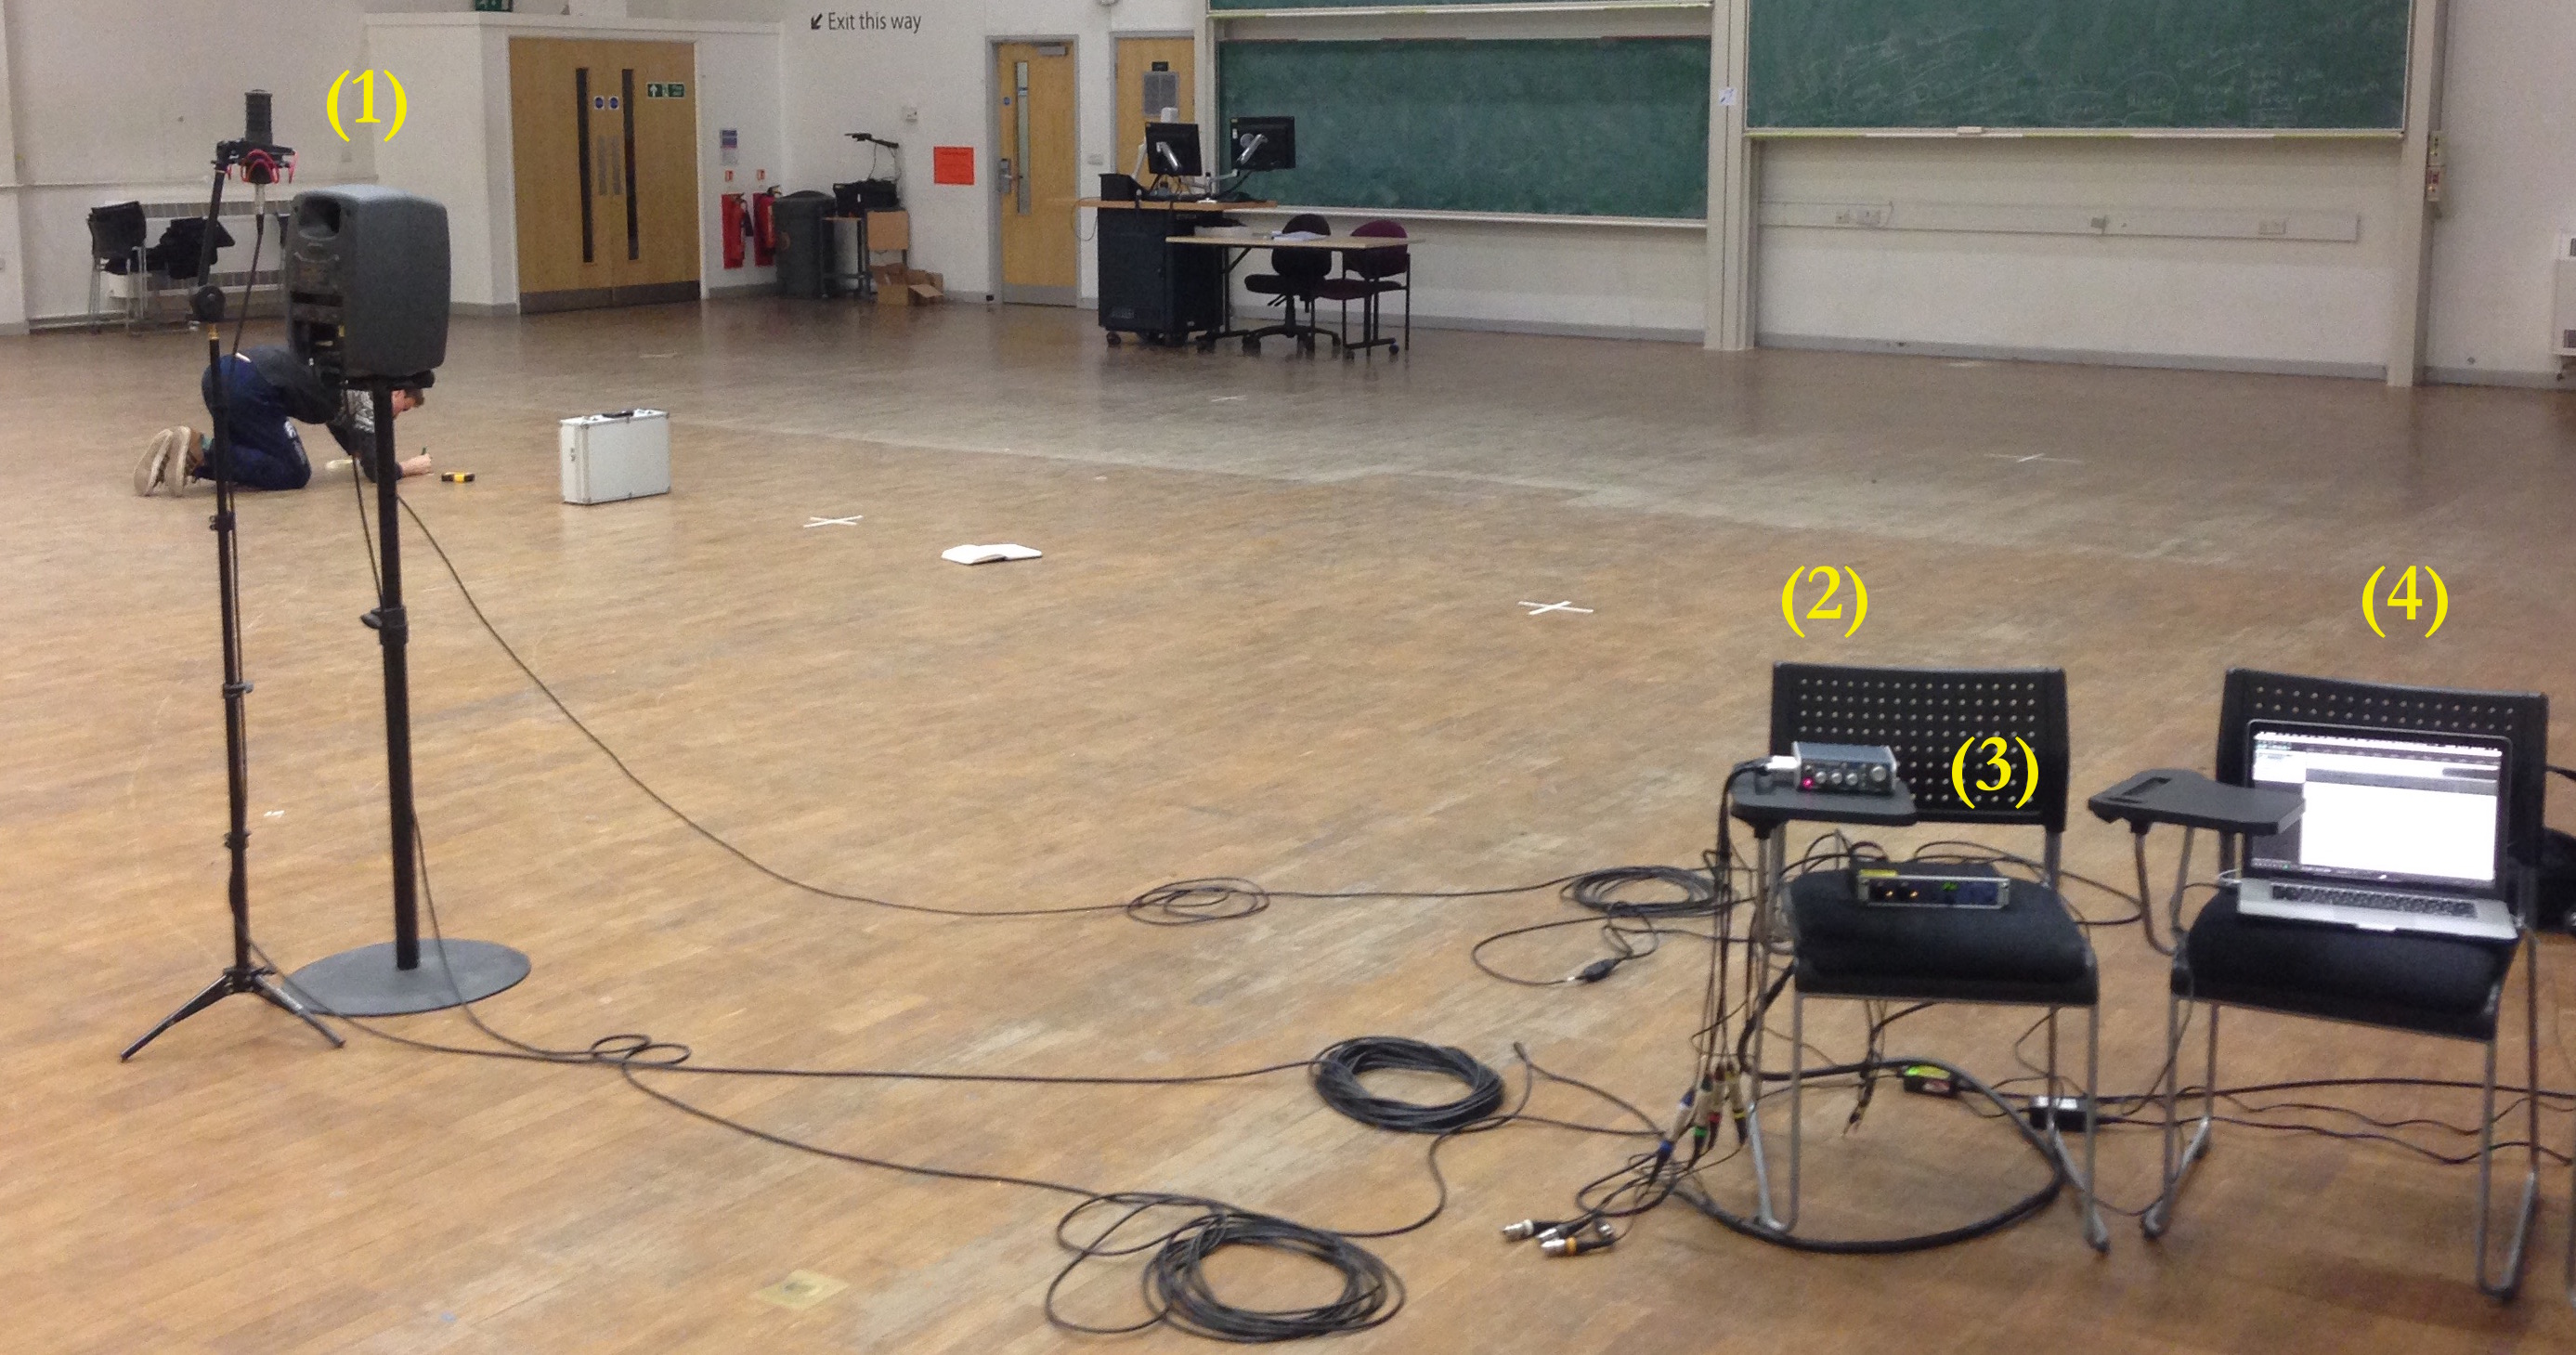
\includegraphics[scale = 0.14]{Sections/Implementation/RealRIRs/images/realRIRSetup_edit.jpg} 
				\caption{Real \ac{RIR} measurement set up. \textbf{(1)}: Sound source and receiver set up \textbf{(2)}: Soundfield interface \textbf{(3)}: Fireface UXC audio interface \textbf{(4)}: Mac running Reaper to output sinusoidal sweep and record B-format input}
				\label{realRIRSetup}
			\end{center}
		\end{figure}

	%-------------Positions-------------%
	\subsubsection{Positions}

		Four positions within the room were chosen and marked with tape for the \ac{RIR} positions shown in figure~\ref{rirPositions} where:

		\begin{center}
			\begin{tabular}{l| c c c c}
				Position & (1) & (2) & (3) & (4) \\
			Coordinates [x(m), y(m)] & [9,9] & [4.5,9] & [2,9] &  [10.13,1.46]\\
			\end{tabular}
		\end{center}

		%-------------Real RIR Positions Image-------------%
		\begin{figure}[H]
			\begin{center}
				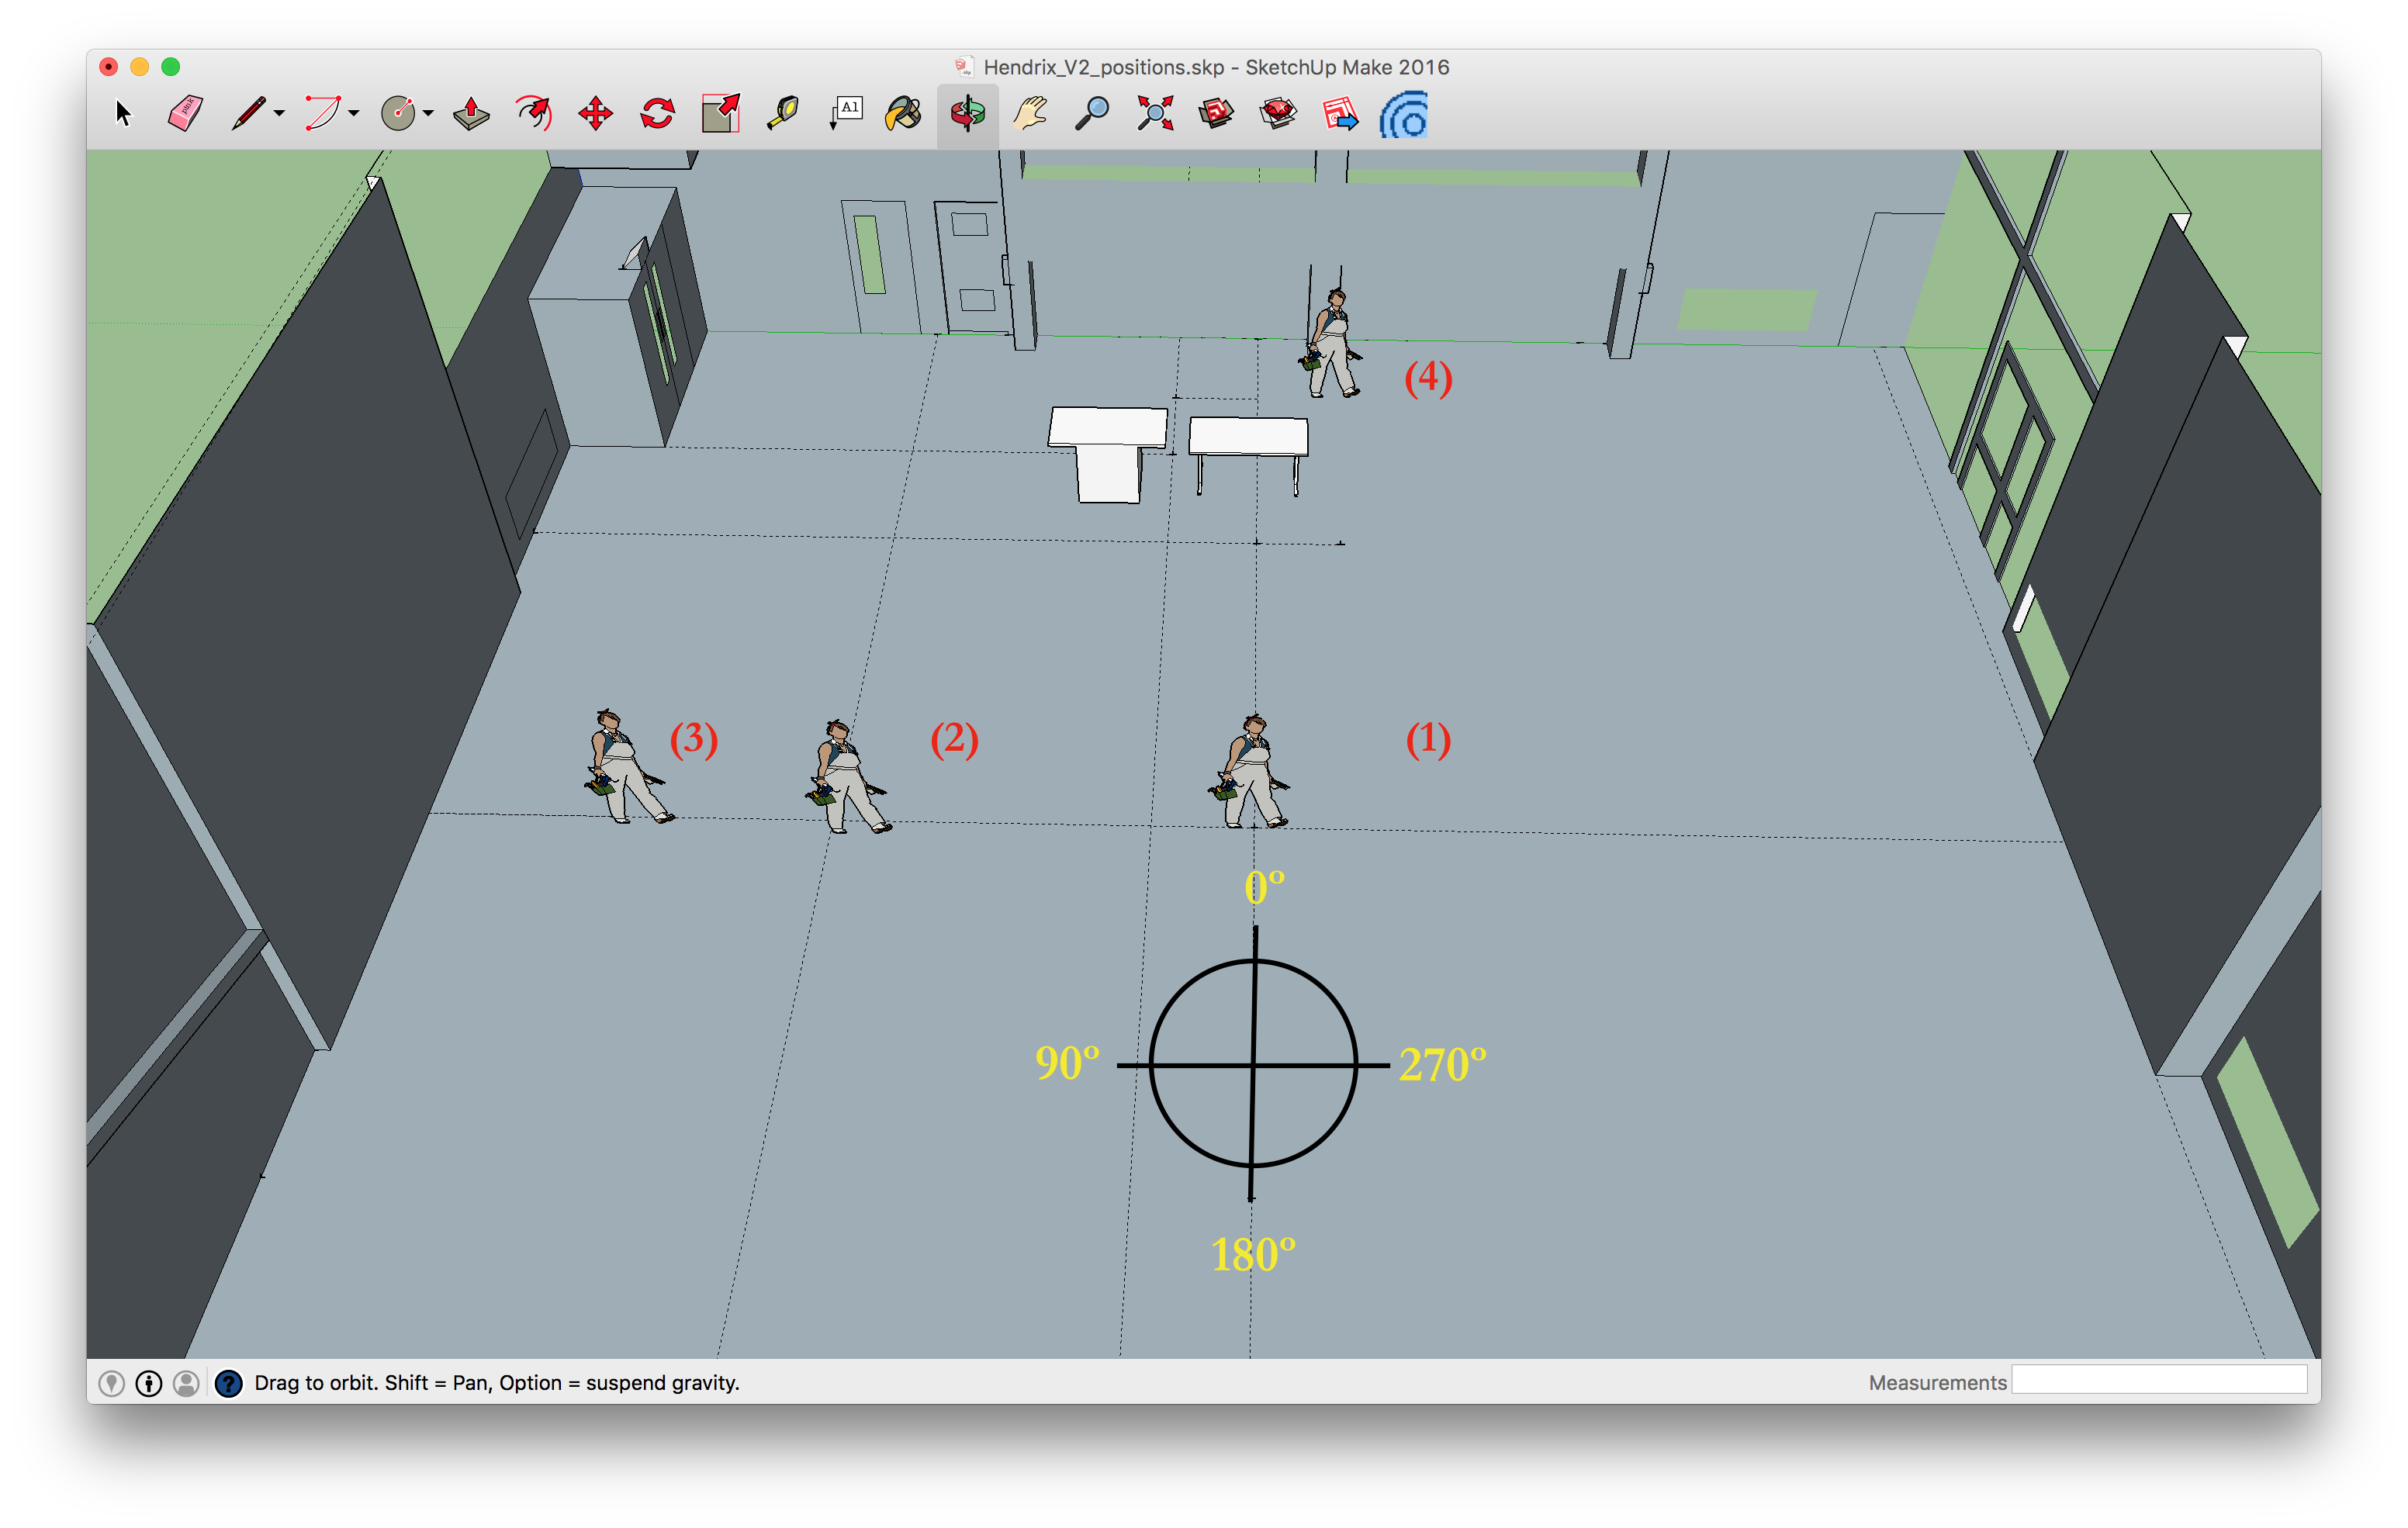
\includegraphics[scale = 0.3]{Sections/Implementation/RealRIRs/images/Real_RIRs7_editV2.png} 
				\caption{Google SketchUp model showing the positions of where the real \ac{RIR}'s were taken}
				\label{rirPositions}
			\end{center}
		\end{figure}
		% \begin{figure}[ht]
		% 	\begin{center}
		% 		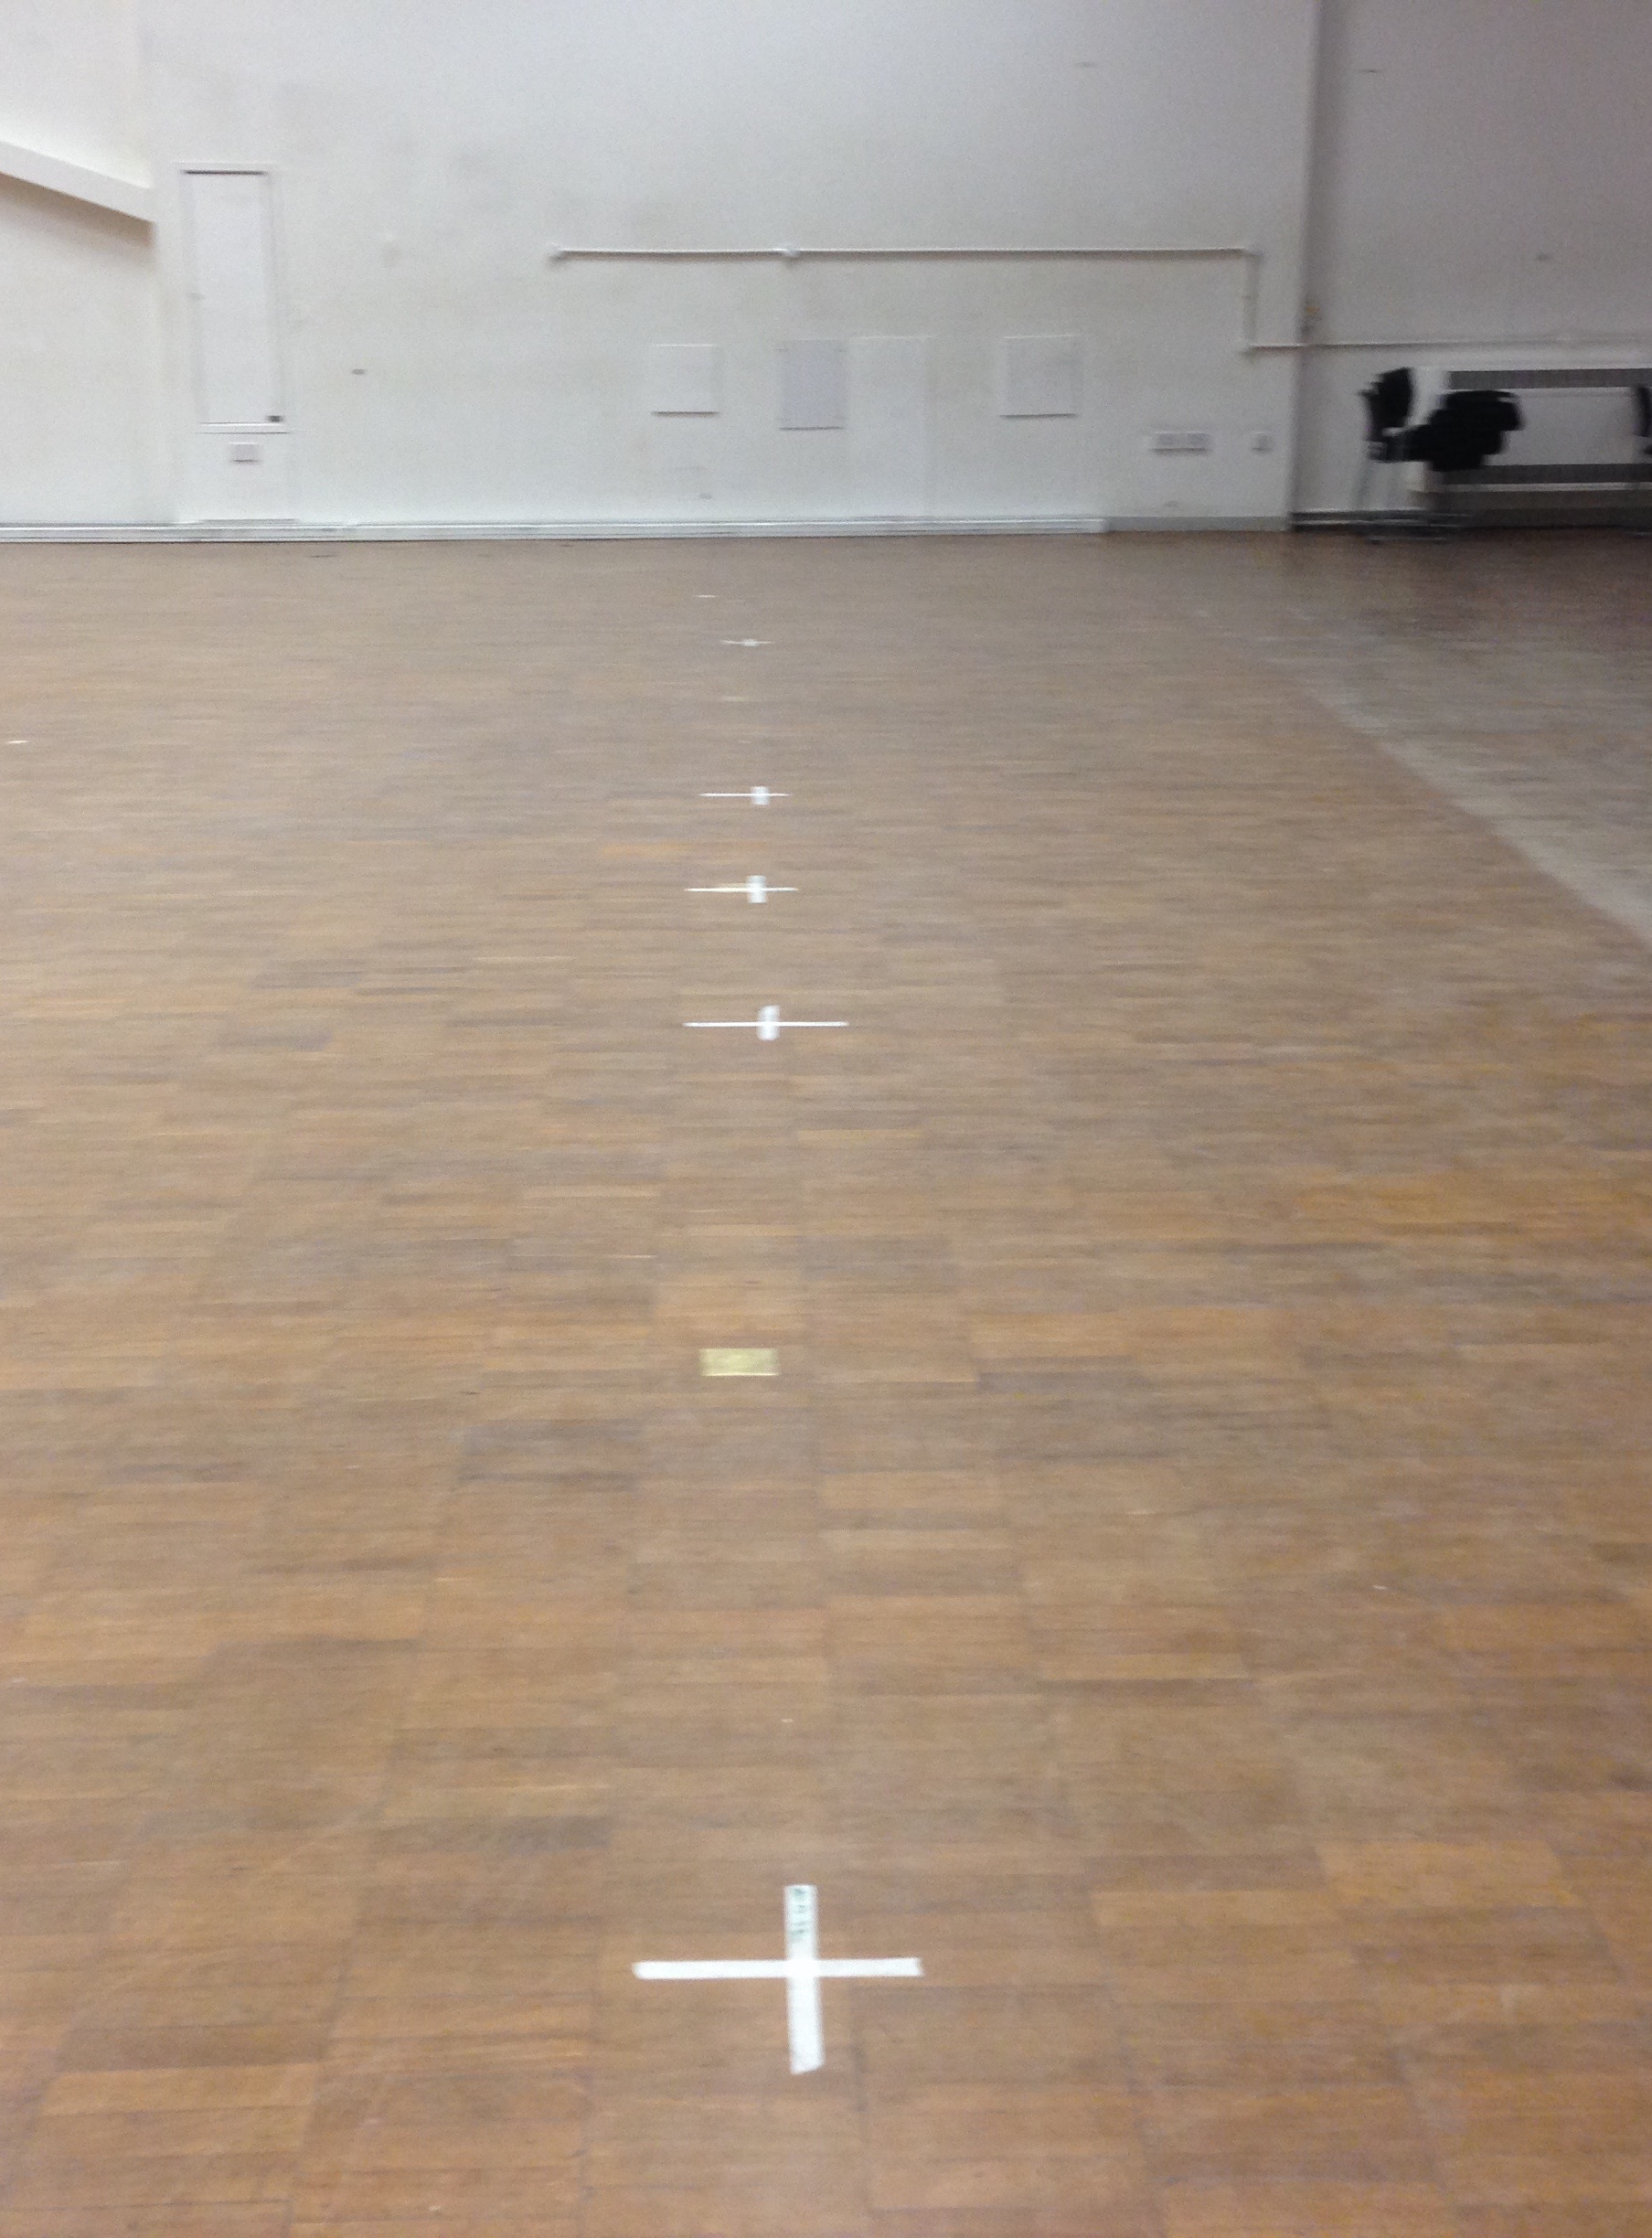
\includegraphics[scale = 0.15]{Sections/Implementation/RealRIRs/images/realRIRTape_edit.jpg} 
		% 		\caption{Google SketchUp model showing the positions of where the real \ac{RIR}'s were taken}
		% 		\label{rirPositions}
		% 	\end{center}
		% \end{figure}

	For each position an \ac{RIR} was taken in four different directions  starting at 0\textdegree~and rotation anti-clockwise 90\textdegree~(anti-clockwise rotation is a standard in Ambisonics) by rotation the sound source and keeping the receiver facing the same direction. This ensures that when the user turns their head in the \ac{VSS} the sound field does not rotate as they do. Once the four directional \ac{RIR} were recorded, the source and receiver were moved to the next marked location with care being taken to make sure the receiver is placed the same distance away from the sound source each time.

	%-------------Measurements-------------%
	\subsubsection{Measurements}
		The sound source signal used was a 15 second long exponentially swept sinusoid ranging from 20Hz to 20kHz with an 8 second padding to ensure that the room could be vacated before the sweep began. The sweep was produced using the Matlab function \texttt{generatesweep.m} taken from the departmental website \cite{sineSweep} which produced both the sinusoidal sweep and an inverse sinusoidal sweep used for deconvolution at a later stage.
		
	\subsubsection{RIR Analysis}

		Once the measurements had been recorded, the first 8 seconds of the files were muted in order to remove noise such as door slams as the room was vacated. Then the signals were deconvolved with an inverse of the sinusoidal sweep to time align the frequency dependant room reflections. This was done using the deconvolution Matlab function \texttt{deconvolve.m} again taken from the departmental website \cite{sineSweep}.

	\subsubsection{Issues}
		Several issues arose when taking the initial \ac{RIR}'s. Simply connection the outputs from the Soundfield converter to the incorrect inputs on the Fireface audio interface meant that the initial recordings contained tracks that were not necessarily recorded in the correct order, i.e the tracks were not recorded as [W, X, Y, Z] but could have been recorded in a possible 24 combinations. This meant that when used to convolve with an audio source, the localisation of the sound source would be incorrect.

		Through observation it was possible to narrow down which order the channels might have been recorded in, however as it could not be 100\% certain the measurements were taken again.

\subsection{RIR Calibration}
	
	As both the real and synthetic \ac{RIR}'s were to be used in the user test, it was imperative that they were calibrated to be the same level to prevent a difference in perception when convolving with an audio signal. As the real \ac{RIR}'s were louder than the synthetic ones and the fact that there were far fewer real \ac{RIR} measurements than synthetic ones, the real measurements were decreased in level to match those produced by Odeon.

	\subsubsection{Matlab}

	In an attempt to perfectly reduce the level of the real \ac{RIRs} to match those of the synthetic ones, using Matlab, a multiplier was calculated by taking the RMS level of both the real and synthetic \ac{RIRs}:

	\begin{lstlisting}
		Multiplier = RMS(real)/RMS(synthetic)
	\end{lstlisting}

	\ac{RIR}'s from the centre of the room were taken and used to calculated the multiplier. Figure~\ref{calRMS} shows the plots of both of the original \ac{RIR}'s (top = real, centre = Odeon) and the calibrated version of the real \ac{RIR} (bottom). As it can be seen, the peaks of the real \ac{RIR} fall within the same range as the synthetic \ac{RIR}. However, when these \ac{RIR}'s were convolved with an audio sample taken from OpenAir \cite{singingSample} (sing44.wav) \textbf{[LINK TO SAMPLE]}, it still sounded significantly louder than that of the synthetic RIR convolved with the same audio sample.

	This can be heard in audio examples: \textbf{calRMSConv.wav and odeonConv.wav [LINK]}


	%-------------RMS calibrated RIR Image-------------%
	\begin{figure}[H]
		\begin{center}
			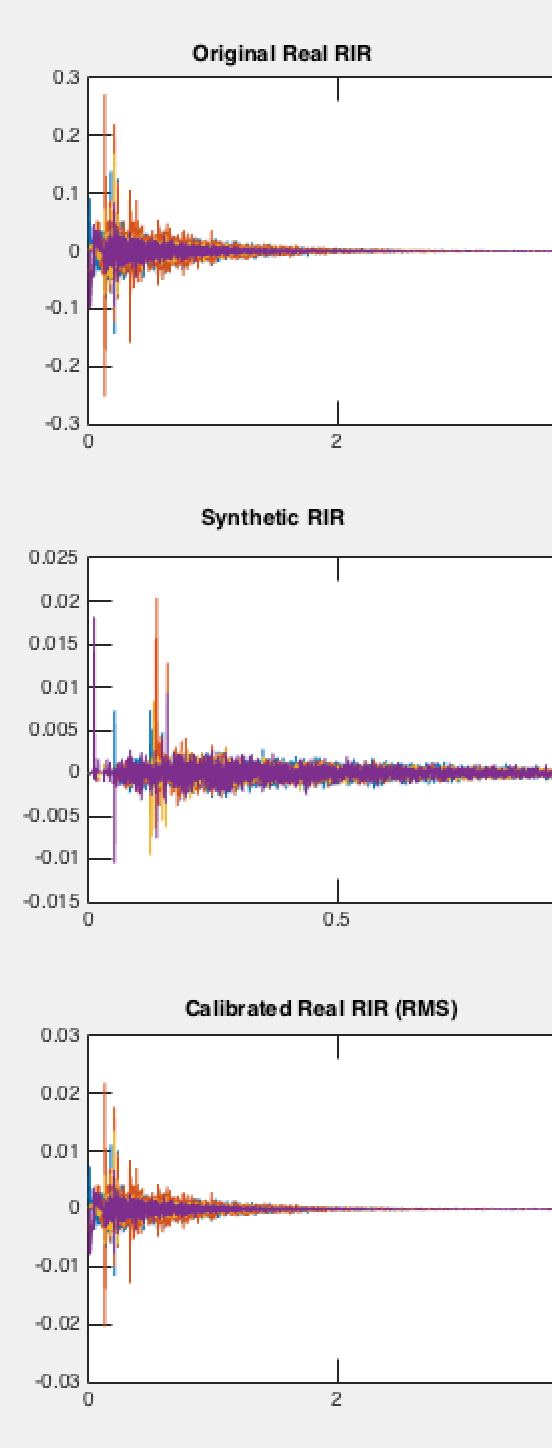
\includegraphics[scale = 0.3]{Sections/Implementation/RealRIRs/images/calibration/CalRMS_RIR_edit2.png} 
			\caption{Plots of the original real \ac{RIR} (top), the synthetic \ac{RIR} (centre) and the calibrated real \ac{RIR} (bottom) using the multiplier calculated using the RMS ratio value showing that the peaks of the calibrated \ac{RIR} sit approximately within the same range as the synthetic \ac{RIR}}
			\label{calRMS}
		\end{center}
	\end{figure}

	As can be seen in figure~\ref{calRMSsing}, the peaks in the signal convolved with the calibrated RIR are approximately twice as large as those in the synthetic RIR convolved with the sample thus is perceived as louder.

	%-------------RMS calibrated Convolved Image-------------%
	\begin{figure}[H]
		\begin{center}
			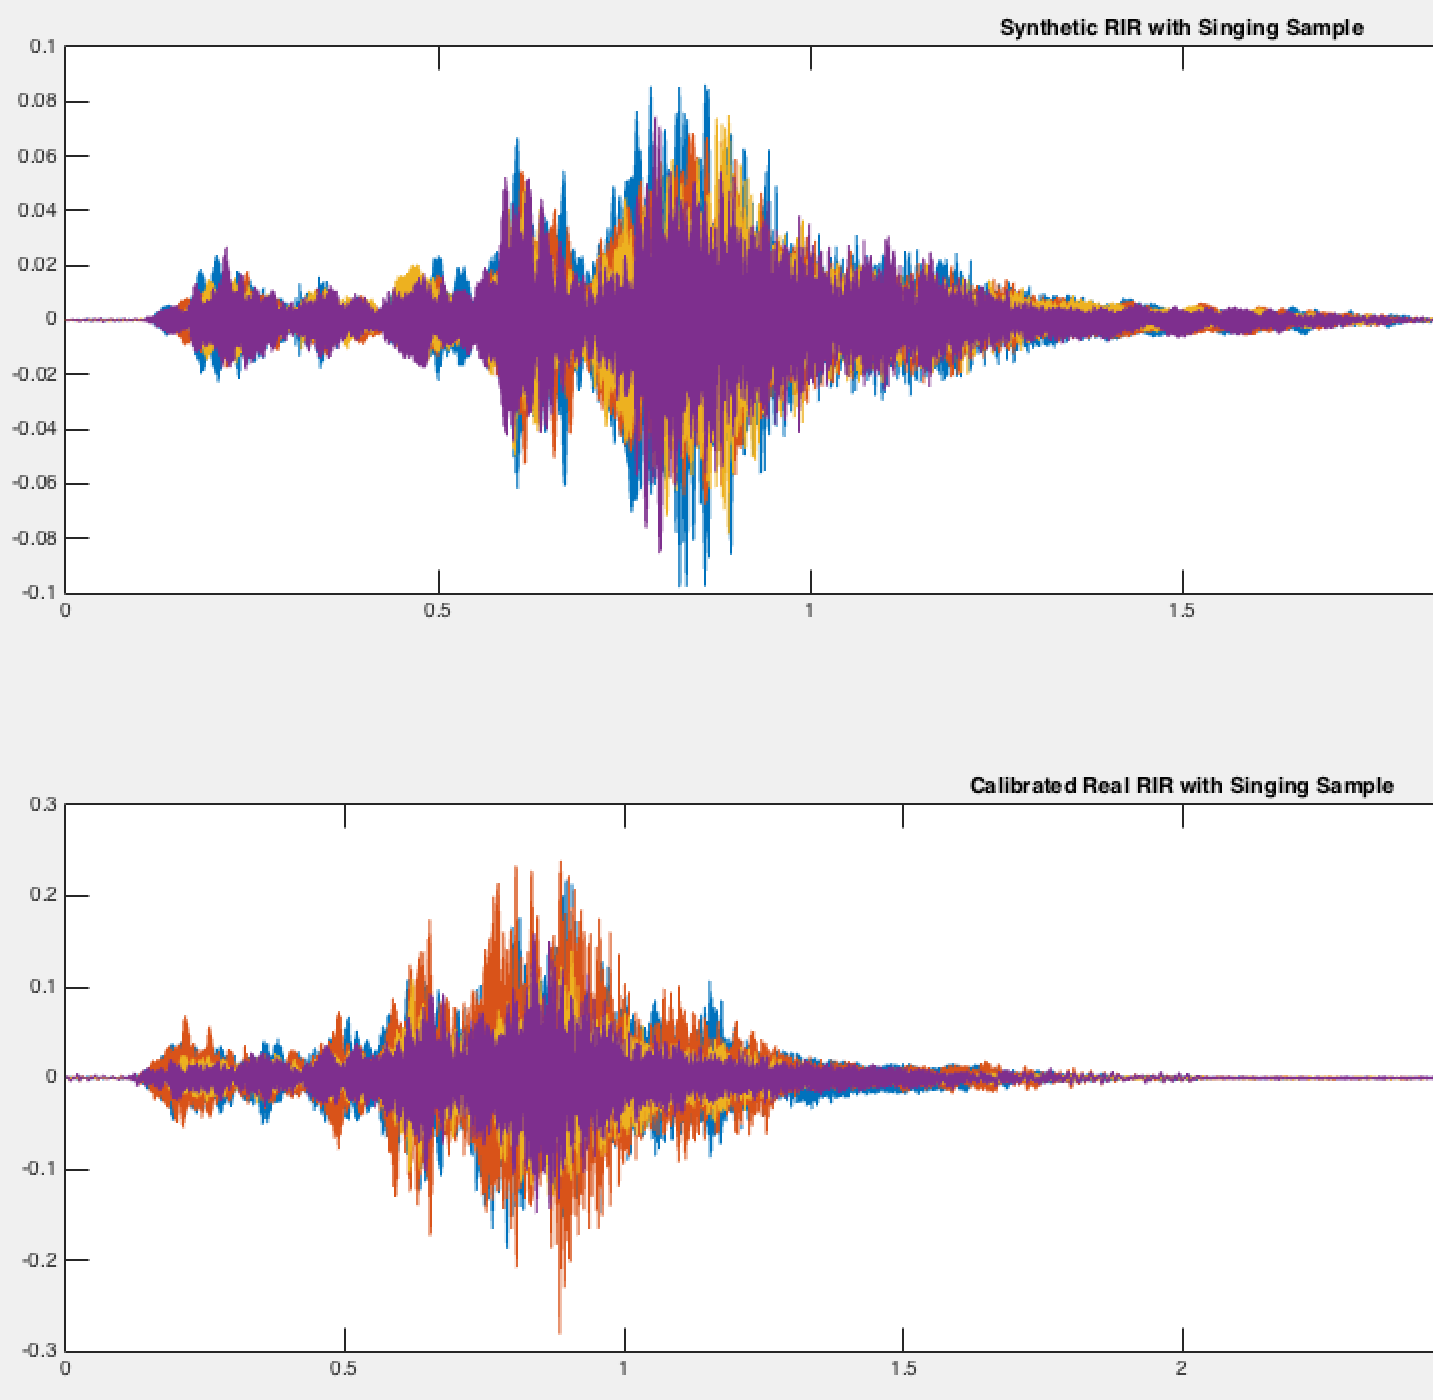
\includegraphics[scale = 0.3]{Sections/Implementation/RealRIRs/images/calibration/CalRMS_Sing_edit.png} 
			\caption{Plots of the synthetic \ac{RIR} (top) and the RMS calibrated real \ac{RIR} (bottom) convolved with an anechoic audio sample showing that the speaks of the calibrated \ac{RIR} convolved sample sit approximately in the range double that of the synthetic \ac{RIR} convolved sample, thus is perceived as louder.}
			\label{calRMSsing}
		\end{center}
	\end{figure}

	Several manual values for the multiplier were tried starting from 0.7 down to 0.2. It was found that a value of 0.3 can the closest level similarity. Figure~\ref{calMan} shows that the level of the manually calibrated RIR falls within values half the magnitude of those found in the synthetic RIR. As the RMS calibrated audio sample shows that its magnitude sits within value twice as large as the synthetic \ac{RIR} sample, now that the peaks of the manually calibrated \ac{RIR} sit within half the synthetic \ac{RIR}'s range, it makes sense that the audio samples now approximately lay within the same range, as can be seen in figure~\ref{calMansing}.

			%-------------Manually calibrated RIR Image-------------%
	\begin{figure}[H]
		\begin{center}
			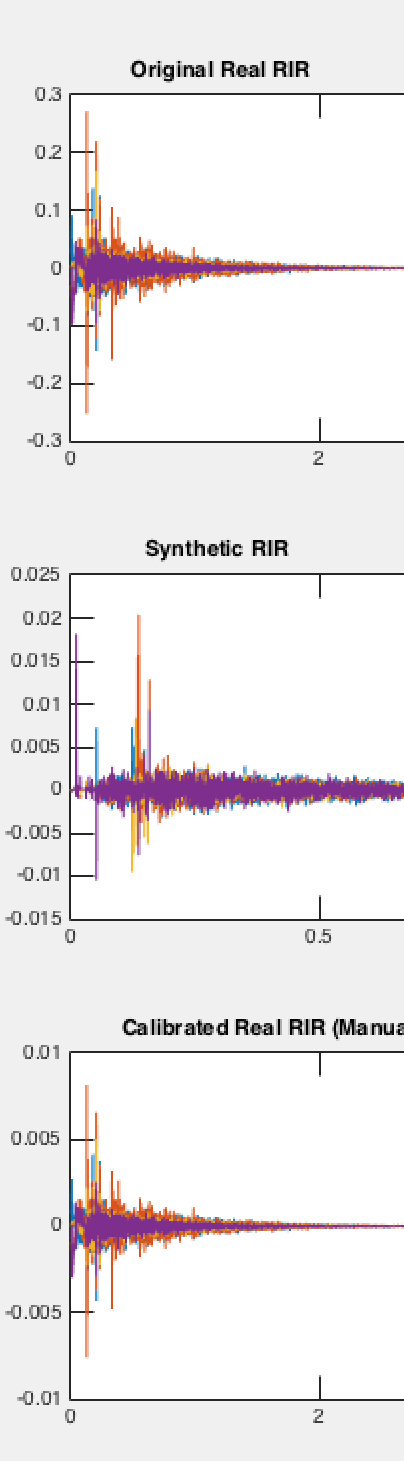
\includegraphics[scale = 0.3]{Sections/Implementation/RealRIRs/images/calibration/CalMan_RIR_edit.png} 
			\caption{Plots of the original real \ac{RIR} (top), the synthetic \ac{RIR} (centre) and the \textit{manually} calibrated real \ac{RIR} (bottom) showing that the peaks of the manually calibrated \ac{RIR} sit within half of the range of the synthetic \ac{RIR}.}
			\label{calMan}
		\end{center}
	\end{figure}

	%-------------Manually Calibrated Convolved Image-------------%
	\begin{figure}[H]
		\begin{center}
			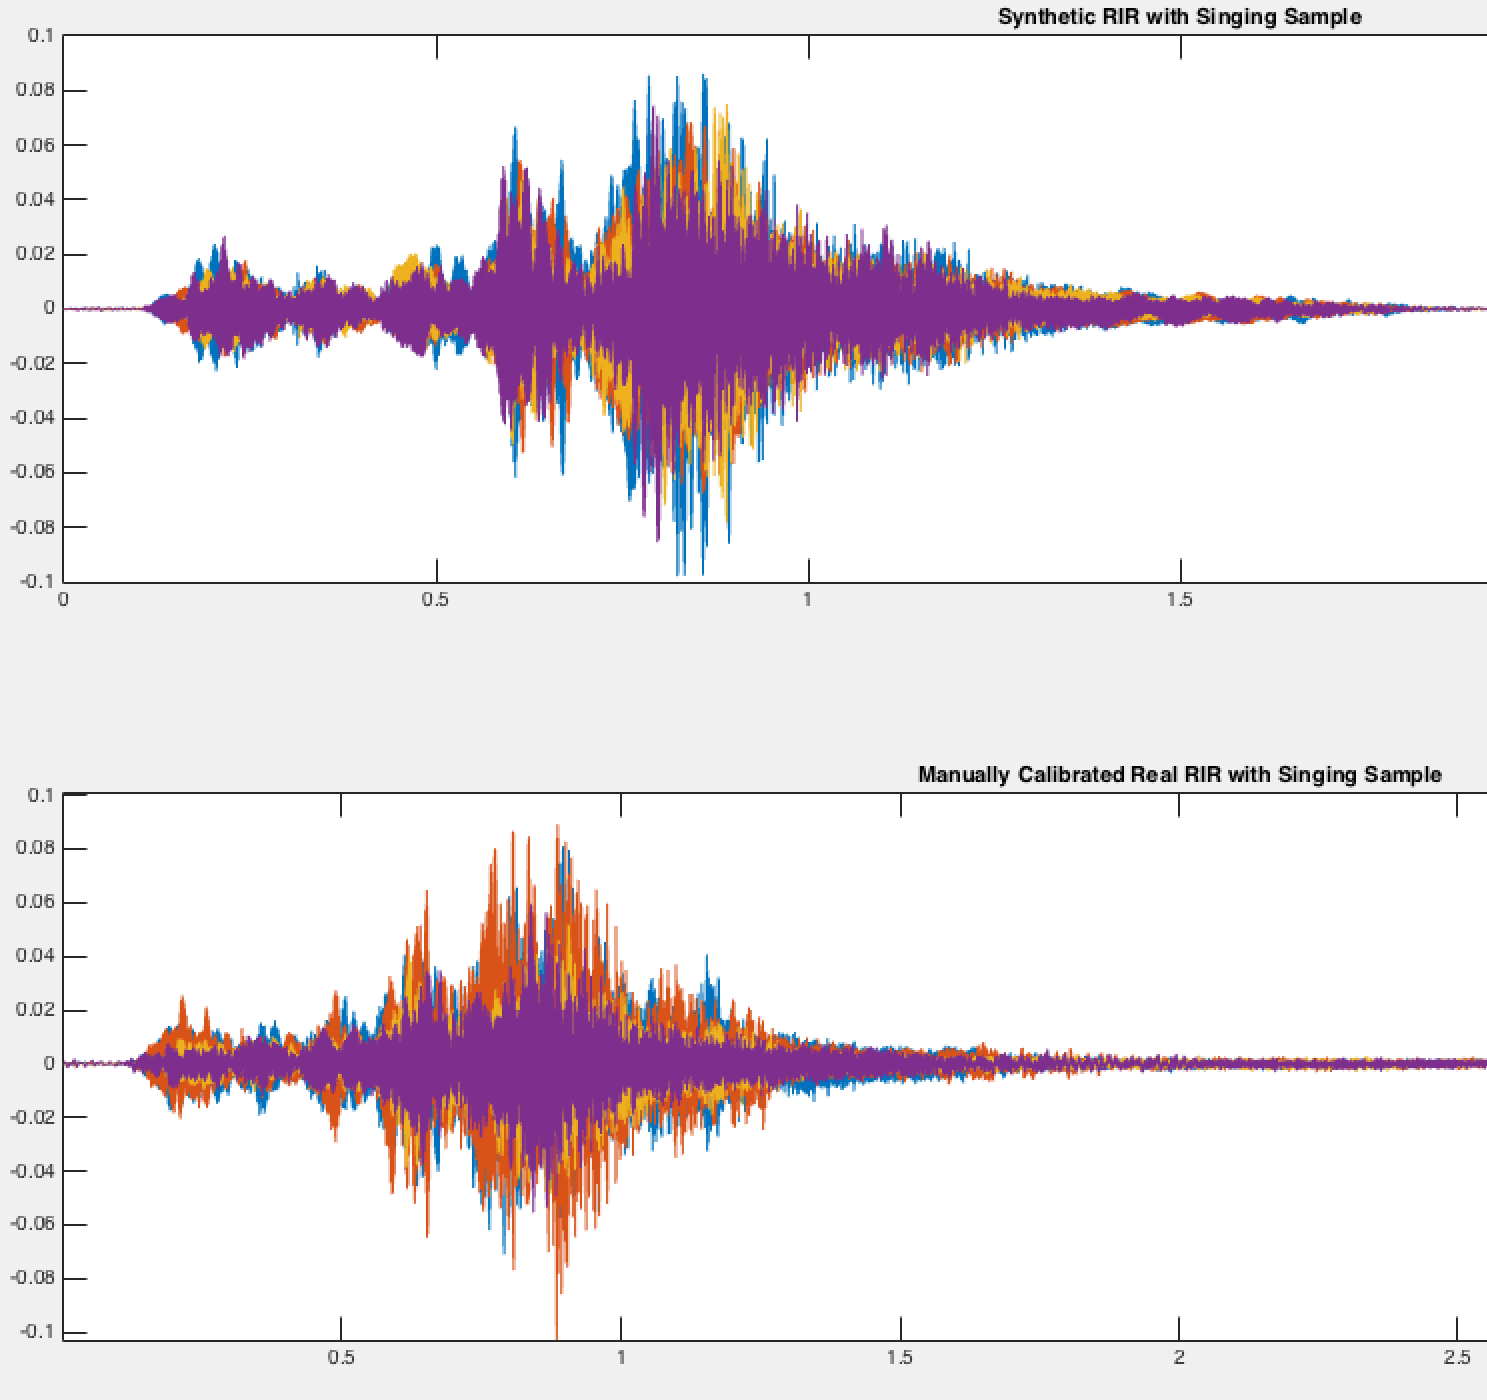
\includegraphics[scale = 0.3]{Sections/Implementation/RealRIRs/images/calibration/CalMan_Sing_edit.png} 
			\caption{Plots of the synthetic \ac{RIR} (top) and the RMS calibrated rel \ac{RIR} (bottom) convolved with an anechoic audio sample showing that the speaks of the calibrated \ac{RIR} convolved sample sit approximately in the range double that of the synthetic \ac{RIR} convolved sample.}
			\label{calMansing}
		\end{center}
	\end{figure}

	After listening to the convolved audio file more closely, it could be heard that the tail of the reverb seemed to increase in volume, producing what sounded like a `swelling' effect. Figure~\ref{pulse} shows the reverb tail of the manually calibrated convolved audio samples, there small pulses can be seen (mostly in the channel shown in yellow). Further investigation did not reveal the cause of the pulsing, though it was found that it occurred every 0.05s, making it a 20Hz pulse. The effect of the pulse can be heard in the audio sample: pulseExample.wav \textbf{[LINK HERE]}.

	%-------------Pulse Image-------------%
	\begin{figure}[H]
		\begin{center}
			\includegraphics[scale = 1]{Sections/Implementation/RealRIRs/images/calibration/cal_pulse.png} 
			\caption{Reverb tail of the audio sample convolved with the manually calibrated \ac{RIR} showing a pulse like pattern.}
			\label{pulse}
		\end{center}
	\end{figure}

	As the cause of the problem could not be uncovered within the time allocated, a solution was found.

	\textbf{Matlab file used: calibrateALL.m}

	\subsubsection{Reaper}

		All of the real \ac{RIR} files were imported into Reaper and send through a bus to a master channel in order to normalise all \ac{RIR}'s evenly. These were then compared by ear to a synthetic \ac{RIR} and manually level matched. The closest match was by reducing the level of the real \ac{RIR}'s by 28.6dB. Though this method is less accurate, it prevented any unwanted errors in the signal such as those caused by using Matlab.

%--------------------------Link Testing--------------------------%
% There a link like: \href{/SuportingFiles/doc.pdf}{Audio!}

% \href{file:/SuportingFiles/index.html}{Fuck it}

% \href{run:/SuportingFiles/.}{DirectoryFUCK}

% \HREF{run:/SuportingFiles/.}{Directory}

% \href{file:/SuportingFiles/CalMan_RIR.png}{Image}

\end{document}